\graphicspath{{Images/}}

\section{Ejercicio 1}\label{cap:ej1}
\subsection{Consigna}
    Dados dos procesadores $P_0$ y $_1$ el tiempo que tarda en enviarse un mensaje desde $P_0$ hasta $P_1$ es una función de la longitud del mensaje $T_{comm} = T_{comm(n)}$, donde n es el número de bytes en el mensaje. Si aproximamos esta relación por una recta, entonces
    $$T_{comm} = l = \frac{n}{b}$$
    donde \textbf{l} es la “latencia” y \textbf{b} es el “ancho de banda”. Ambos dependen del hardware, software de red (capa de TCP/IP en Linux) y la librería de paso de mensajes usada (MPI). Para determinar el ancho de banda y latencia de la red, escribir un programa en MPI que envíe paquetes de diferente tamaños y realice una regresión lineal con los datos obtenidos. Obtener los parámetros para cualquier par de procesadores en el cluster. Comparar con los valores nominales de la red utilizada (por ejemplo, para Fast Ethernet: \textbf{b} $\approx$ 100Mbit/sec, \textbf{l} = O(100$\mu$ sec)).

\subsection{Resolución}
Adjunto la resolución del ejercicio uno debajo. Sin embargo, recomiendo visualizarlo en el repositorio de GitHub de este trabajo \cite{justog220_practica-car_2023}.

\subsubsection{Implementación con MPI}
\lstinputlisting[language=C++]{codigos/main1.cpp}

\subsubsection{Ejecución en cluster}
Habiendo resuelto la codificación del ejercicio, me conecté al cluster por SSH y envié mi código. Una vez allí, lo compilé y establecí distintos parámetros para correrlo con SLURM (\ref{fig:scriptSLURM}).

\begin{figure}[H]
    \centering
    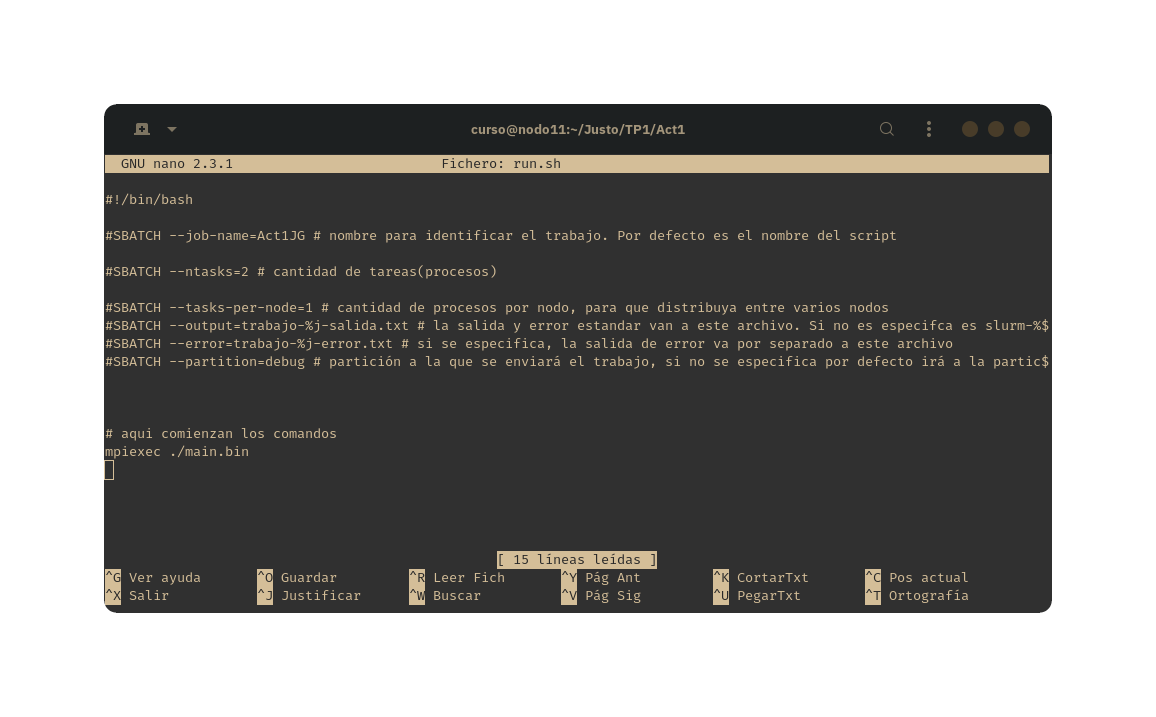
\includegraphics[width=0.60\textwidth]{Images/ej1/Captura desde 2023-08-30 14-22-23.png}
    \caption{Script run.sh para SLURM}
    \label{fig:scriptSLURM}
\end{figure}

Habiendo establecido los parámetros procedo a correrlo con:

\begin{lstlisting}
sbatch run.sh
\end{lstlisting}

Este comando me devuelve el identificador de la tarea lanzada y gestionará su ejecucioón en base a la disponibilidad de cómputo.

Luego observé el estado de mi tarea(\ref{fig:squeue}) con:
\begin{lstlisting}
squeue -l
\end{lstlisting}

\begin{figure}[H]
    \centering
    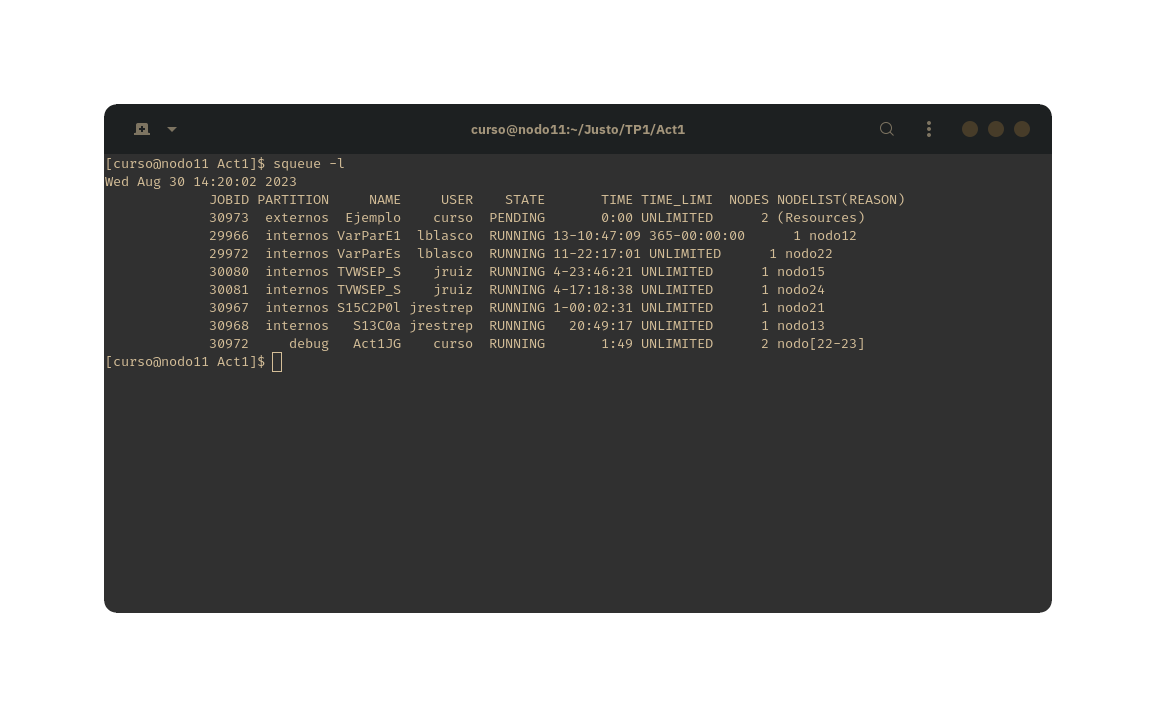
\includegraphics[width=0.60\textwidth]{Images/ej1/Captura desde 2023-08-30 14-20-39.png}
    \caption{Tarea corriendo}
    \label{fig:squeue}
\end{figure}

Finalizada su ejecución, copié la salida en mi dispositivo y realicé el análisis descripto a continuación

\subsubsection{Análisis de resultados}
Habiendo obtenido los datos de latencias realicé un procesamiento de datos con Python, análisis que recomiendo ver en el repositorio de GitHub \cite{justog220_practica-car_2023}.

La salida de mi código fue pensada como valores separados por coma para luego manipularlo facilmente como un archivo de tipo csv. Por ello simplemente hice uso de la librería \textit{pandas} para cargarla como DataFrame y luego analizarla. 

Al momento de la implementación decidí que la medición se realizara 10 veces para poder representar mejor los tiempos para cada tamaño. Por ello tuve que hacer un preprocesamiento para promediarlos. Habiendo realizado esto, obtuve la siguiente tabla:

\begin{table}[H]
\centering
 \begin{tabular}{|c | c|} 
 \hline
    Tamanio & Tiempo \\
    \hline
    1 & 0.000023 \\
    2 & 0.000021 \\
    4 & 0.000021 \\
    8 & 0.000022 \\
    16 & 0.000022 \\
    32 & 0.000022 \\
    64 & 0.000022 \\
    128 & 0.000022 \\
    .. & \\
    8192 & 0.000023 \\
    16384 & 0.000024 \\
    32768 & 0.000027 \\
    65536 & 0.000031 \\
    131072 & 0.000039 \\
    262144 & 0.000054 \\
    524288 & 0.000082 \\
    1048576 & 0.000139 \\
    ... & \\
    1073741824 & 0.120231 \\
 \hline
 \end{tabular}
 \caption{DataFrame obtenido tras la carga de datos}
\label{tab:ej1}
\end{table}

Con los datos ya cargados y promediados hice un análisis exploratorio de los datos con un ScatterPlot \ref{fig:scatterej1}.

\begin{figure}[H]
    \centering
    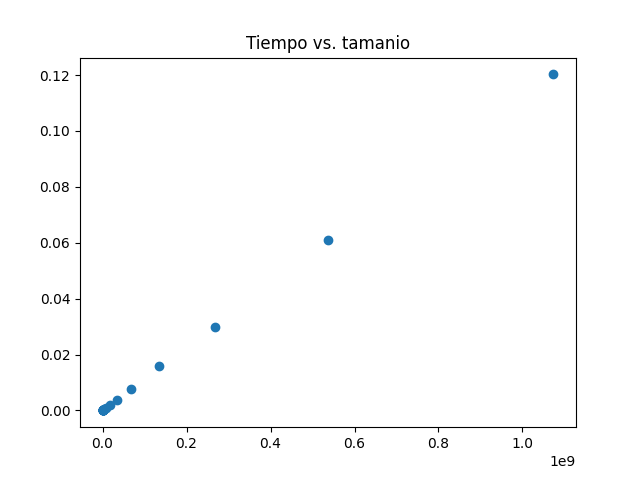
\includegraphics[width=0.60\textwidth]{Images/ej1/scatterej1.png}
    \caption{Scatter plot de los datos}
    \label{fig:scatterej1}
\end{figure}

Se puede observar que los datos parecen tener una relación lineal. Luego, importé de la libreria \textit{SciKit Learn} los módulos necesarios para hacer una regresión lineal con mis datos.

\begin{lstlisting}
    from sklearn.linear_model import LinearRegression

    reg = LinearRegression()

    x = dfProm[["Tamanio"]]
    y = dfProm["Tiempo"]
    
    reg.fit(x, y)
\end{lstlisting}

Teniendo ya la recta que mejor se ajusta a mis datos, la plotee junto al Scatter Plot (\ref{fig:regej1})

\begin{figure}[H]
    \centering
    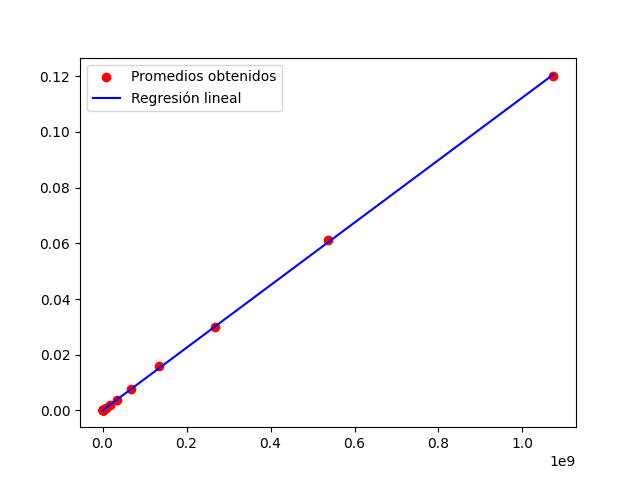
\includegraphics[width=0.60\textwidth]{Images/ej1/reglinej1.png}
    \caption{Datos y la recta ajustada a ellos}
    \label{fig:regej1}
\end{figure}

Habiendo obtenido la regresión lineal, calculé la latencia como la ordenada:

\begin{figure}[H]
    \centering
    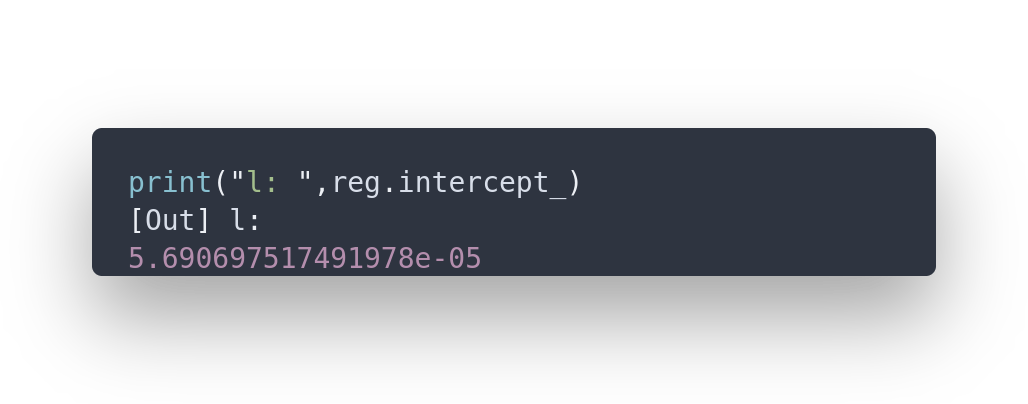
\includegraphics[width=0.60\textwidth]{Images/ej1/intercept.png}
    \caption{Latencia de la red}
    \label{fig:latej1}
\end{figure}

$$l \approx 5,7$$

Luego, de la ecuación de la recta despejé el ancho de banda:
$$b = \frac{n}{T_{comm} - l}$$

Con los datos del DataFrame calculé este dato:
$$b \approx 8905586616.9$$
